%A more indepth look at how the system is designed with UML- and class-diagrams. Directed towards developers. Start with subsubsection here.

A more indepth look at how the system is designed with UML- and class-diagrams. It is divided into two main sections for the server and clients. The client section contains the different clients. After that follows the server section that is divided into different parts that makes up the whole server. 

\section{Clients}
Here is an explanation of the  different client system designes.
\subsection{Desktop}
\subsubsection{Overview of the desktop client}
The \term{UML} diagram in \refer{fig:des_uml-overview} describes the whole desktop client.
\begin{figure}[htb!]
%	\addScaledImageVertical{0.172}{des_UML.jpeg}
	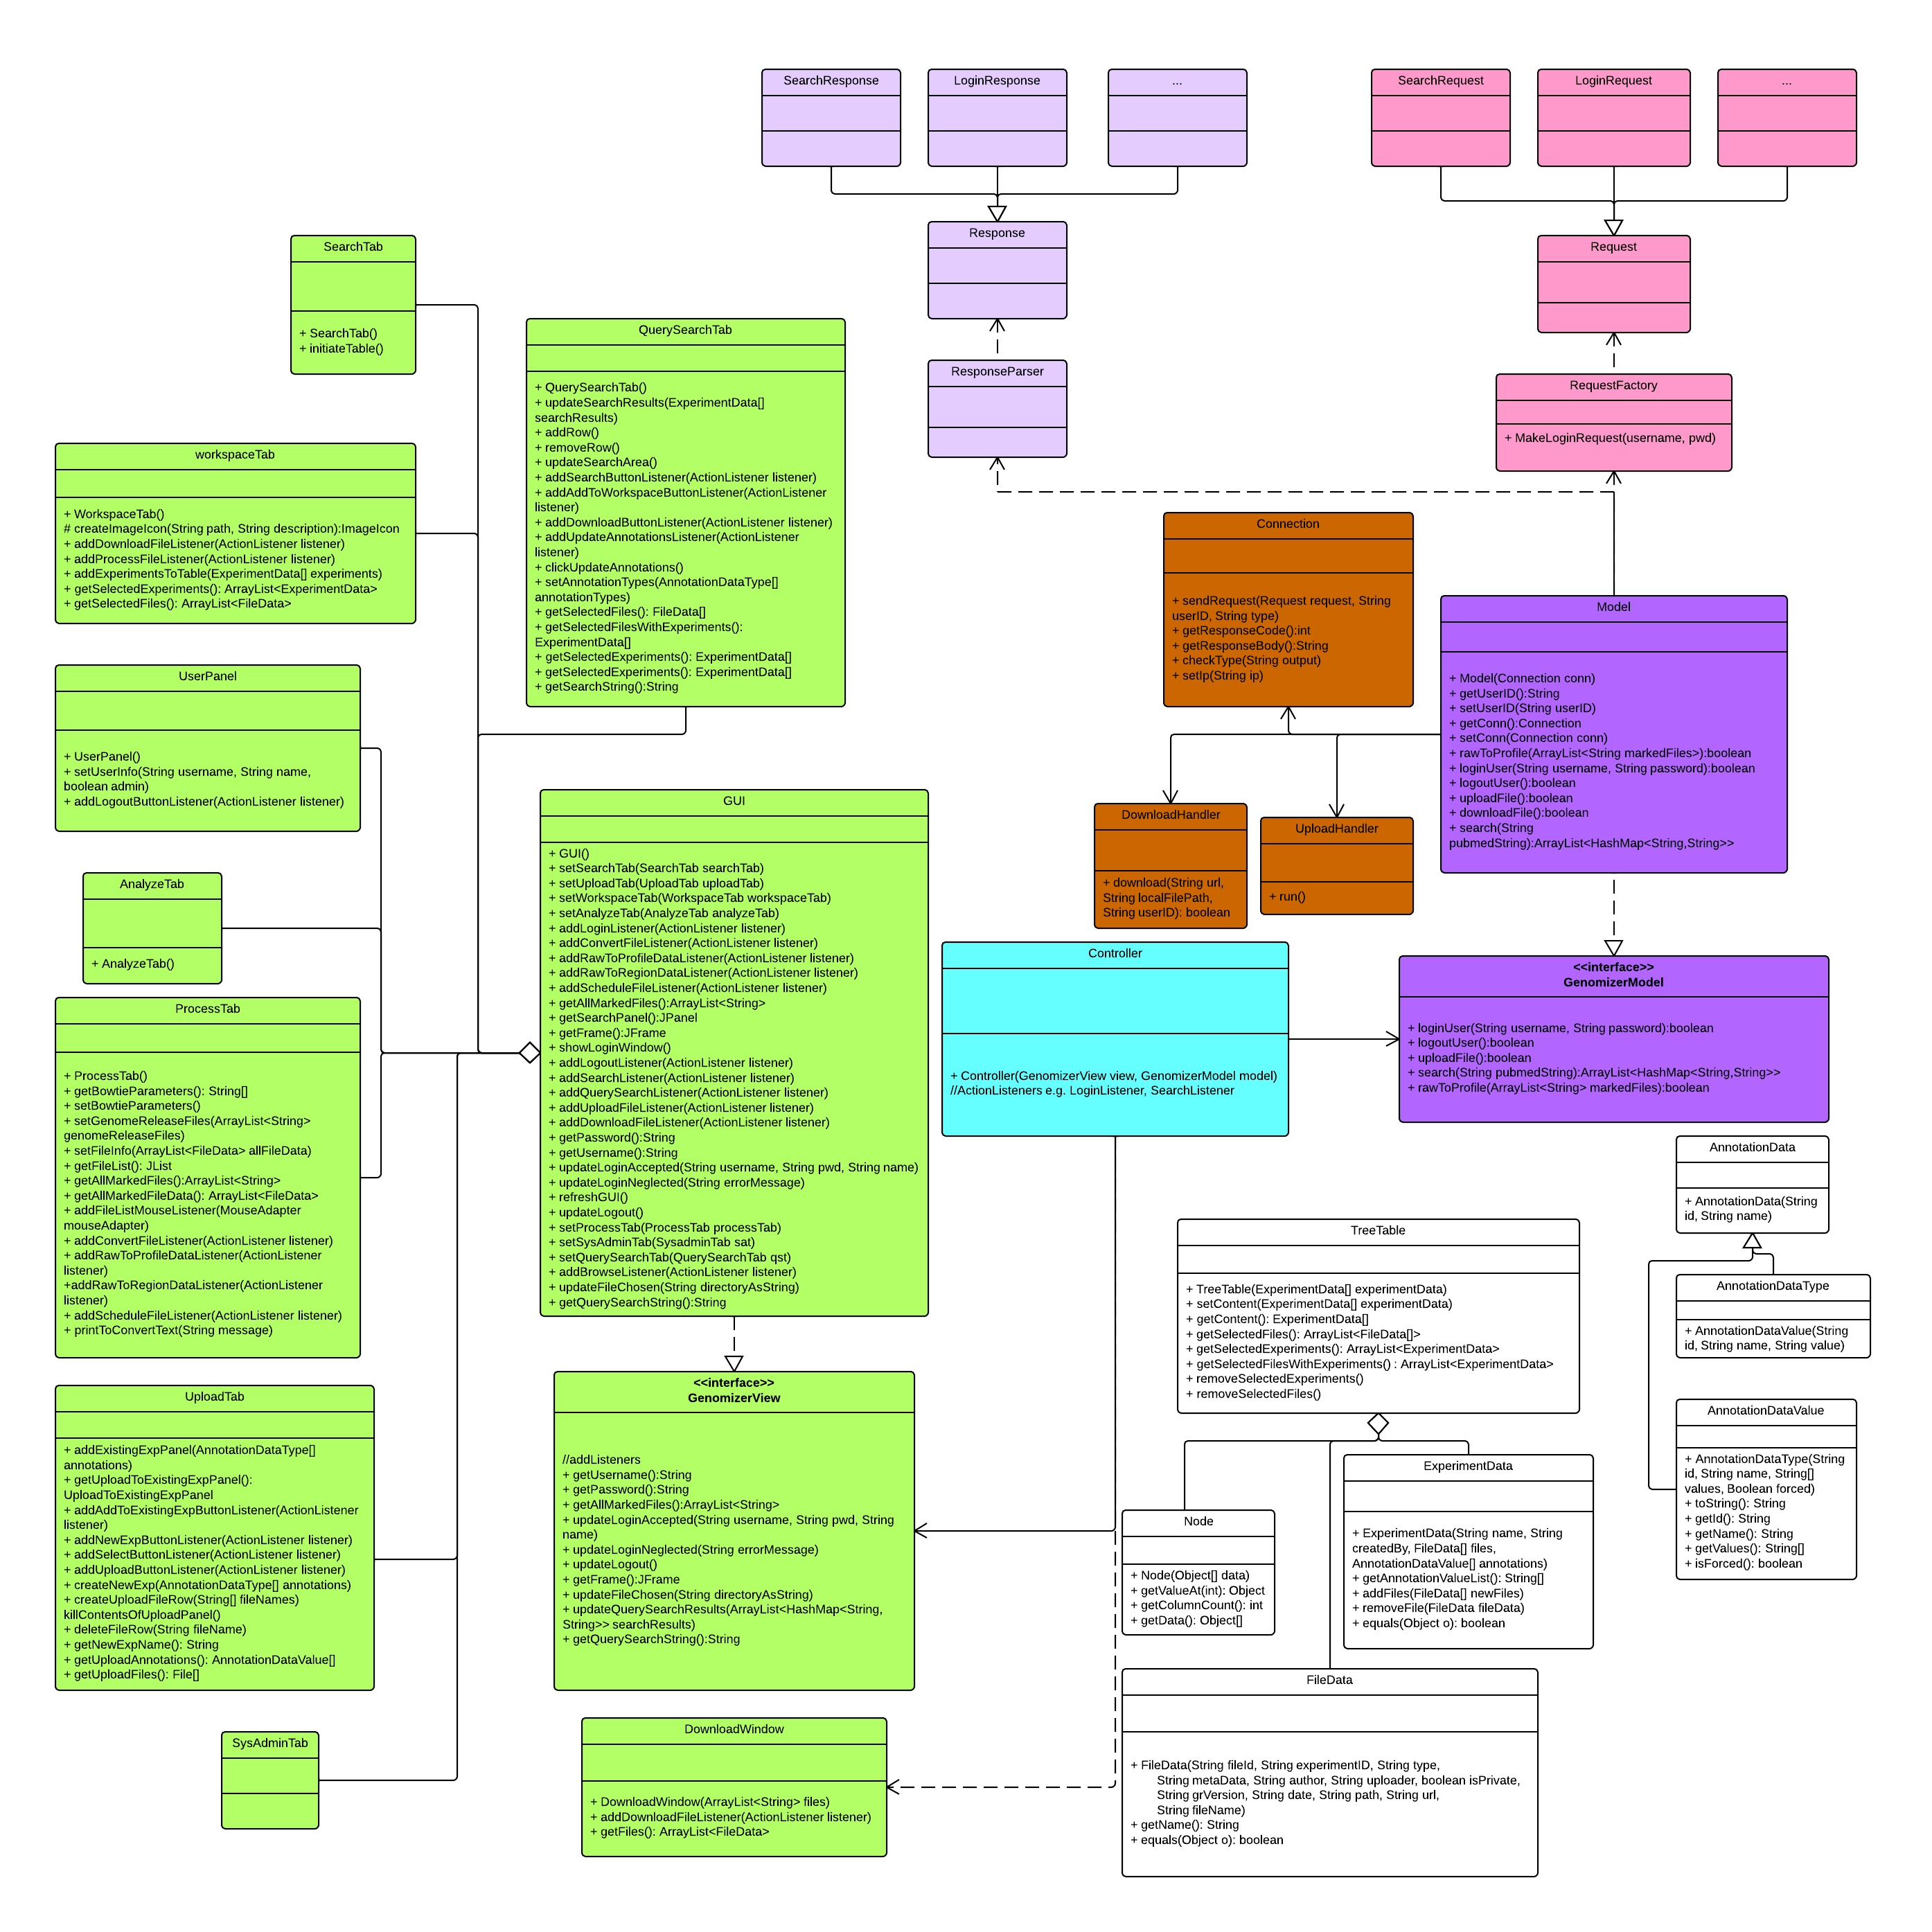
\includegraphics[width=\textheight,height=\textwidth, angle=90]{des_UML.jpeg}
	\caption{UML diagram over the desktop client}
	\label{fig:des_uml-overview}
\end{figure}

\subsubsection{View}
The view of the \appName\ Desktop client is constructed around tabs. There are 6 different tabs. These are \term{Search}, \term{Process}, \term{Upload}, \term{Workspace}, \term{Analyse} and \term{Administration}. In this version the \term{Analyze} tab is not used.

Each tab in the view is represented by its own java class. The \term{QuerySearchTab} class which represents the search tab can display both a search view and a results view. It uses the \term{QueryBuilderRow} class to construct the rows in the query builder which is used to construct search queries. The \term{QueryBuilderRow} class represents a row in the query builder and each row is dynamic and can change accordingly to user interaction.

The \term{UploadTab Class} represents the upload view of the \term{GUI}. It has functionality to both upload a file to an existing experiment (which is separately handled in the UploadExistingExpPanel) and to create a new experiment to upload files to.

The \term{ProcessTab} class represents the process view in the \term{GUI}. It contains a list where files to be processed can be stored and buttons and eight parameters for initiating the processing.

The \term{WorkspaceTab} class consists of six buttons and a \term{TreeTable} that holds all the experiments and their data. The buttons are: Delete from database, Remove selected, Download selected, Analyze selected, Browse local files and Process selected. From the workspace, the download function/window is accessible. The \term{DownloadWindow} holds the \term{FileData} to be downloaded and its \term{GUI} consists of a \term{JTable} showing the file names and has JComboBoxes for choosing file format and a download button which opens a JFileChooser to download files.

The \term{AnalyzeTab} Class is not yet implemented.

\subsubsection{Model}
The model part of the system contains method for doing most of the logic in the system. For example there are methods for sending login requests and for downloading files. There are separate classes for downloading and uploading files as well as a class for regular communication with the server called \term{Connection}.

\subsubsection{Requests}
The \term{Request} package contains the \term{Request} class , the \term{RequestFactory} and all the classes that extends the \term{Request} class. \term{Request} is the super class and can make a \term{JSON} package that all the other \term{Request} classes can use. All requests must have a name, type and an \term{URL}, but can consist of more information. For example \term{LoginRequest} also has username and password. \term{RequestFactory} is a class that can create all objects from all types of requests. It is a way to easily create all requests from the same place.


\subsubsection{Response}
This package consists of all types of responses that the server can send to the client-program. There is a class named \term{Response} that all the other response classes extends from. For example there is \term{LoginResponse}, \term{SearchResponse}. All these types of responses has different properties. There is also a class \term{ResponseParser} that can parse the responses so that the important information can be taken out of a \term{JSON}-package. This information can then be used to tell the client program what should happen next in the user interface. 


\subsubsection{Controller}
The controller part of the system consists of \term{ActionListeners} for the different buttons and functionalities in the view. For example there are Listeners for searching, downloading and processing. The Controller class has access to both the view and the model and acts as a middle hand between those two parts of the system. Usually a Listener in the controller reacts upon user input and then modifies the model and gives information about the change to the view.
\FloatBarrier

\subsubsection{Utilites}

There are several classes which represents different data in the system. There are classes for experiment data, file data and annotation data. For example when a search response is received from the server it is parsed into experiment data and the experiment data contains file data and annotation data.

The TreeTable class represents the table which displays experiment data, annotation data and file data in the Search and Workspace tabs. It is specially constructed to handle the data classes and it allows vertical sorting.

\subsubsection{System Administration}
%Till Anna!
The System Administration Tab is developed separeately from the rest of the Desktop GUI, and hence has it's own back end description here. 

\paragraph{Observer observable}
\label{Observer observable}

\begin{figure}[htb!]
\addImage{des_sysadminUML.png}
\caption{Communication UML}
\label{fig:adm_viewmodelcomuml}
\end{figure}

Observer is an interface and Observer is a class, and together they are used to simplify communication. This pattern is used when one object needs to be automatically notified of changes in another object. The observing object has to implement the Observer interface. This interface enforces only the \textit{update()} method which will be triggered every time something changes in the observed object. The Observable on the other hand is a class and any object that wants to be observed has to extend the Observable class. The Observable class has a few methods that can be of use but most important ones are \textit{addObserver()}, which is used to add an observer that will observe this object, \textit{setChanged()} simply sets flag that verifies that this object has changed, and finally \textit{notifyObservers()} that notifies all objects observing this object that something has changed and so triggers their \textit{update()} methods.

This pattern is used for communications between the system administration view and the main controller.

\paragraph{View to controller communication}


When the user requests a state change on the server of any kind, the following steps occur. When the user clicks the button to trigger the request a listener will fetch the data from the GUI and package it into a specific datatype. When finished the listener triggers the \textit{notifyObservers(<object>)} method with the datatype as an argument. Which in turn triggers the \textit{update()} method in the \textit{SendDataObserver} class located in the main controller. The \textit{SendDataObserver} unpacks the data and then calls the model which creates the request.

In \refer{fig:adm_viewmodelcomuml} an example of this communication flow is visible. An example is when a user wants to create a new annotation. Once the user has filled in all the neccesary fields in the new annotations view, the user clicks the 'Create annotation' button (See \refer{fig:adm_desktopgui}). The \textit{AnnotationPopupListener} receives the event and calls the \textit{sendNewAnnotation()} method in the \textit{SysadminController} class. This method then creates an instance of the datatype \textit{AddAnnotationRequest} using the input from the textfields in the \textit{SysadminAnnotationPopup}. Since the  \textit{SysadminController} is an Observable object, it then uses the inherited methods \textit{setChanged()} and \textit{notifyObservers()}. This triggers the \textit{update()} method in the \textit{SendDataObserver} class (which implements the Observer interface and is an inner class of the \textit{Controller} ). The \textit{update()} method only receives an object, so first it verifies that the Object is of the \textit{AddAnnotationsRequest} type, and then extracts the neccesary attributes from the datatype and sends them to the \textit{GenomizerModel} which create the request.





\subsubsection{Annotation}

The annotation tab is implemented in the class \textit{AnnotationsViewCreator} 

\paragraph{Add annotations}
When adding a new annotation which is done from the popup window that is implemented in the \textit{SysadminAnnotationPopup} class, the \textit{AnnotationPopupListener} recives an event. The event is parsed and the \textit{sendNewAnnotation()} method will be executed in the \textit{SysadminController} class. Here the input from the user will be fetched and sent into a new datatype object of \textit{AddAnnotationRequest} (located in the \textit{requests} packet). This object will in turn be sent to the model via the observer observable (see \ref{Observer observable} - Observer observable) design pattern that is implemented. 



\subsubsection{Flow of the system}

The sequence diagram in \refer{fig:des_download-sequence} describes the flow of the system when the user presses the download file button and the diagram in \refer{fig:des_login-sequence} describes how the desktop clients reacts to a login.





\begin{figure}[htb!]
	\addImage{des_downloadsequence.jpeg}
	\caption{UML sequence diagram of downloading a file}
	\label{fig:des_download-sequence}
\end{figure}

\begin{figure}[htb!]
	\addImage{des_loginsequence.jpeg}
	\caption{UML sequence diagram of login}
	\label{fig:des_login-sequence}
\end{figure}
\FloatBarrier

\FloatBarrier
\subsection{Web}
This section describes the design of our system, first with a system overview and then with more indebth information about our tabs.

\subsubsection{How our web application works}
%figure x5
\begin{figure}[ht]
\centering
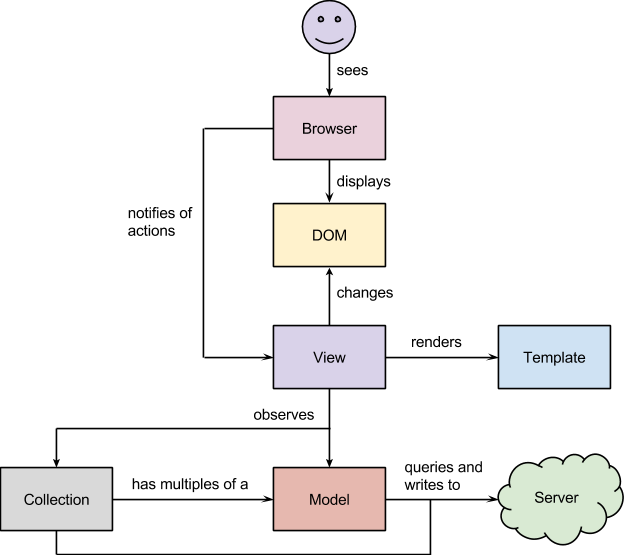
\includegraphics[width=1\textwidth]{web_system_backboneWebapp.png}
\caption{\label{fig:web_system_backboneWebapp}A general build of a backbone webapp.}
\end{figure}

\refer{fig:web_system_backboneWebapp} shows how a backbone\cite{web_1} web application works in general. We have a user, that interacts with a browser. A browser renders the DOM of our web application. How it does this is up to the browser. Different browsers might display it differently. Models and Collections will talk to the server to update themselves. For example, our \textit{Experiments} collection will retrieve experiments from the server and update itself with a call to it’s fetch() method. Out of the components that go into this figure, we are in charge of and only capable of changing a few of these; \textbf{View}, \textbf{Template}, \textbf{Collection} and \textbf{Model}. See the Backbone section of Frameworks in section \ref{sec:web_frame} more information.

\subsubsection{System overview}
%figure 2
\begin{figure}[ht]
\centering
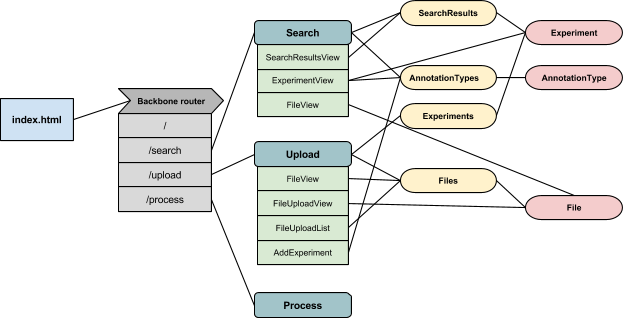
\includegraphics[width=1\textwidth]{web_system_overview.png}
\caption{\label{fig:web_system_overview}Overview of the relations between the different javaScript prototypes in the system.}
\end{figure}

Since our app is built using Backbone\cite{web_1}, our app is divided into the parts \textbf{Misc}, \textbf{Views}, \textbf{Collections} and \textbf{Models}. In \refer{fig:web_system_overview}, we can see the system overview. The \textbf{views} are the parts in green, the \textbf{collections} the parts in yellow and the \textbf{model} the parts in red. The parts in grey represent the router which belongs in our Misc category. It is responsible for rerouting links. For example, when a user clicks the search tab, the router navigates to /search, but instead of loading the whole /search over the page we are currently on, our router will open our search tab below our navigation bar. The \textbf{Misc} category also holds our Main.js, which is in charge of setting up and starting the app.

\subsubsection{Search}
The search tab has three views, the main one being \textit{Search}, which acts as a container for the \textit{SearchResultsView}and holds the search input field and the various buttons displayed. The \textit{SearchResultsView} handles rendering the annotations and the \textit{ExperimentViews}, where one \textit{ExperimentView} is created for every experiment returned from a search. The actual data retrieved is stored, by experiment, in \textit{Experiment models}. To organise this data, we have a collection to contain all the experiments retrieved, called \textit{SearchResults}.
 
%figure bla bla/lalalallala
\begin{figure}[ht]
\centering
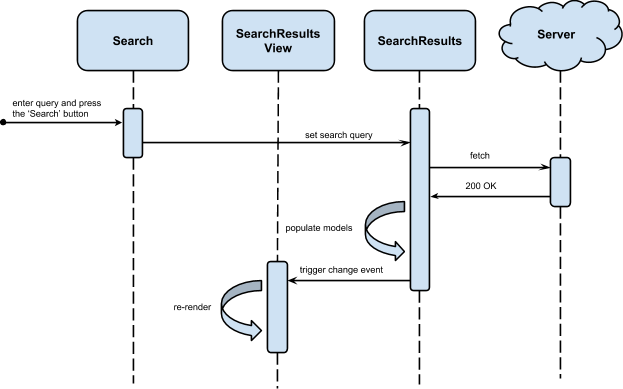
\includegraphics[width=1\textwidth]{web_system_sequenceDiagram.png}
\caption{\label{fig:web_system_sequenceDiagram}a sequence diagram showing what happens when a user enters a valid search query and results are fetched.}
\end{figure}

In \refer{fig:web_system_sequenceDiagram} is a simple sequence diagram for the search tab. If a user enters a query in the search field and then presses the search button, the \textit{Search} view will update the \textit{SearchResults} collection to have a new query. Once \textit{SearchResults} has a new query, it will try to fetch search results corresponding to the query from the server. If successful, new experiment models for every experiment retrieved will be created and set in the \textit{SearchResults} collection. \textit{SearchResults} then triggers a ‘change’ event that \textit{SearchResultsView} listens to. When that event occurs, \textit{SearchResultsView} knows that \textit{SearchResults} has been changed, and re-renders itself.


\subsubsection{Upload}
The upload tab has three main views, the main one being Upload, which acts as a container for the ExperimentView’s and holds the search input field and the various buttons displayed. Each ExperimentView handles rendering the AnnotationsForm and the FileUploadList, where one ExperimentView is created for every experiment the user inputs. The actual annotation data and files input by the user is stored, by experiment, in Experiment models. To organize this data, we have a collection to contain all the experiments input, called Experiments.
\subsubsection{Process}
To be announced.
\FloatBarrier
\subsection{Android}
This section describes the architectural design of the Android application. All coded functionality is described in this section, inluding the functionality that is not fully integrated. 
\subsubsection{Class descriptions}\label{sec:and_classdescription}
This section focuses on the functionality of each class.

The connection between the classes labeled model can be seen in \refer{fig:and_umlmodel} while the other classes can be seen in \refer{fig:and_uml}
	\begin{figure}[h]
		\addImage{and_UML_model_sprint2.jpg}
		\caption{Android UML of model}
		\label{fig:and_umlmodel}
	\end{figure}  
\begin{figure}[h]	\addImageVertical{and_UML_android_sprint2.jpg}
		\caption{Android UML without model}
		\label{fig:and_uml}
	\end{figure}  
    \FloatBarrier
\subsubsection{Android activities} 
Activities are used as frames to display various fragments. For anything to be displayed it must be a part of a fragment that is a part of an activity. Each activity used in this application extends the class SingleFragmentActivity which has the purpose of creating a new fragment of an arbitrary type that displays a single fragment. This means that in its current state the application contains one fragment per activity and each fragment described in this section is coupled with an activity
\subsubsection{Fragment Class: LoginFragment}
This fragment will be the first view the user sees when the application is started, it allows the user to specify username and password. ComHandler \ref{sec:and_class_comhandler} is then used to send and validate the login request. If the username and password are incorrect the user will be informed through an android toast explaining what happened. Likewise if the server cannot be reached.

A successful login will start the SearchListFragment \ref{sec:and_class_search}.
\subsubsection{Fragment Class: SearchListFragment}\label{sec:and_class_search}
Handles the search-view for the \appName\ app, the annotations that can be chosen are downloaded from the server and they are, as such, dynamic.
\subsubsection{Fragment Class: ExperimentListFragment}
This fragment handles the displaying of search results to the user. The fragment includes a ListView with an ArrayAdapter set to it. An OnItemClickListener is used to detect when the user is selecting an item in the list and is currently starting FileListActivity \ref{sec:and_class_filelist} when a list item is selected. This fragment receives a HashMap with search values from SearchListFragment \ref{sec:and_class_search} and when activity is starting an ASyncTask is started to send and receive search results from the server through the ComHandler \ref{sec:and_class_comhandler} class. When an experiment is selected from the list the file names belonging to that experiment is sent to FileListFragment \ref{sec:and_class_filelist} that will display the file information. 
\subsubsection{Fragment Class: FileListFragment}\label{sec:and_class_filelist}
This fragment displays all files associated with a chosen experiment. The fragment is using three ListViews, one for each data type. The data types that are available are: raw, region and profile. Each list element will show the name of the data file and have a checkbox connected to it. A custom ArrayAdapter is used to handle checkbox interaction and displaying information to the user. There is option to select multiple files in the view by checking several checkboxes. The file names displayed are the ones currently available from the server for each available experiment.
\subsubsection{Model Class: ComHandler}\label{sec:and_class_comhandler}
Is a static object that is called by the fragments in the view to gain access to the models different functions. At this stage the ComHandler can be used to login, search for files and to request raw to profile conversions, although the latter is not yet integrated. The url that ComHandler tries to communicate with can be changed with a public method which makes it possible to implement a way for the user to change server.
\subsubsection{Model Class: Communicator}
Intended to manage the sending and receiving of messages between the server and the application using a http connection.
\subsubsection{Model Class: MsgFactory}
Creates the JSON messages that can be sent to the server.
\subsubsection{Model Class: MessageDeconstructor}
Interprets JSON messages and returns appropriate information.
\subsubsection{Model Class: GenomizerHttpPackage}
Used to store the body and status code of an http-response.
\subsubsection{Model Class: GeneFile}
Used to store and transfer the information of a genome file.
\subsubsection{Model Class: Annotation}
Used to store and transfer one or several annotations and their value.
\subsubsection{Model Class: Experiment}
Used to store and transfer information about an experiment.
\subsubsection{Model Class: ProcessingParameters}
Used to simplify the transfer of parameters in a processing request.

\FloatBarrier
\subsection{iOS}
System design for the Genomizer iOS application. The  system is designed using the model-view-controller principle. Each view is controlled by its own controller class.
\begin{figure}[ht]
\addScaledImageVertical{0.3}{ios_UML.png}
\caption{UML diagram .}
\label{fig:ios_UML}
\end{figure}

\refer{fig:ios_UML} gives an overall image of the system design. Some classes are excluded from the figure due to making it easier to get an overall idea of the system. The controller classes of the table cells and some other controller classes are not illustrated in the diagram. The non-excluded are explained below:

\FloatBarrier
\subsubsection{DataFileViewController}
Controlls the File view presented in \refer{fig:ios_files}. It contains a referens to an experiment and lists all its files in a table.

\subsubsection{SearchResultController}
Controller class for the Search Results view presented in  \refer{fig:ios_searchResult}. It configures the table which holds the information about the experiments a search resulted in. An ExperimentDescriber is used to generate a description of the experiments.

\subsubsection{ExperimentDescriber}
Generates a description of an experiment using annotations chosen by the user.

\subsubsection{Experiment}
A class that contains all information related to an experiment.

\subsubsection{ExperimentFile}
Is a class that contains information about a file from an experiment.

\subsubsection{ExperimentParser}
A class that parses experiment information from a NSDictionary to an Experiment object.

\subsubsection{SearchViewController}
Controller class for the Search view, see \refer{fig:ios_search}. It checks which annotation-fields are used and tells the JSONBuilder to generate a corresponding search query when the user presses the search button. The class also contains a advanced search to allow the user to manually enter search queries. 

\subsubsection{Connection}
A class that sends and receives JSON objects to and from the server.

\subsubsection{JSONBuilder}
A class that can create diffrent JSON requests.

\subsubsection{Selected files}
The selected files controlls the selected files view shown in \refer{fig:ios_selectedFiles}. The selected files class contains information about files saved by the user. It has a method that can make convertion possible. 

\FloatBarrier
\section{Server}
The system design of the different parts of the server.
\subsection{Communication}
The server system is based around HTTP, where clients send requests on a non-persistent connection and the server responds to these requests. All communication is initiated by the client and the server has no way of contacting clients except when responding to a request. 

Clients send requests to the communication part of the server first. When a request is picked up by the server, the request is parsed and a command is created depending on the request. The command then communicates with the other parts of the server in order to get or input relevant data. 

To identify clients a unique token is used, which is generated when a user logs in. The token is sent back to the client, and the client must include this token with all following requests. Since there is no persistent connection between the client and the server this token is the only way for the server to identify the sender of any given request. The token is also used to prevent unauthorized requests from being executed on the server.

Most commands are executed immediately when the server gets a request, and the result is sent back to the client when the command is finished. This happens when for example searching the database. 

The commands implemented for the server are:

\begin{itemize}
	\item $login$
	\item $search$
	\item $annotation$
	\item $experiment$
	\item $file$
	\item $process$
\end{itemize}

The $login$ command can take either a $'POST'$ method or $'DELETE'$ method, depending on if the user wants to log in or log out. 

$Search$ is used for searching for experiments in the database. Results will display all experiments which match the search query, and the user can chose o expand these experiments in order to view the containing files. 

The $annotation$ command can be used to modify and view annotations associated with experiments. The server can respond to a $'GET'$ request with an array of all possible annotations currently in use in the database. There is also possible to add new annotations, update the values for an annotation or delete a complete annotation field. 

Clients can get information about a specific $experiment$ by using a $'GET'$ together with this command. The server will respond with information about the experiment aswell as information about all the files associated with the experiment. Clients can also add, modify and delete experiments. 

An experiment contains $file$s which can be uploaded with this command. A $'POST'$ will let the client upload a file to a specific experiment. Clients can also download, modify and delete files. When a client downloads a file, the communication part of the server is never contacted. This is because a download URL is already present in the file on the client side. Therefore no contact is needed with the communication part of the server, but instead the file system server takes care of the request. 

In order to convert files, the client can send the command $process$. This will convert specific raw files into profile files.
\FloatBarrier
\subsection{Conversion}
The Genomizer service needs to be able to convert, process and visualize data. This chapter explains how this is done in the system.

\begin{figure}[h]
\addImage{con_UMLsprint2.jpeg}
\caption{Classdiagram for Process}
\label{con_UML}
\end{figure}
	
As can be seen in \refer{con_UML} the RawToProfileConverter extends the Executor class. When a call comes to the ProcessHandler it then starts the correct convertion which right now only can be a raw to profile convertion.


\subsubsection{Executor}
The executor class, as seen in figure 5.2.1, is an abstract superclass that is an entity that is able to execute various commands. The executor class is able to run programs as well as scripts. In order to run scripts and programs the executor has a parse-function that parses a string into separate arguments. \newline

\begin{itemize} 
\item executeCommand
\begin{itemize}
\item ExecuteCommand is a private method that is being used by the executeScript, executeProgram and executeShellCommand methods. Firstly a processBuilder is used to ensure a safe way to execute commands, after that the working directory is set and the error output stream is merged with the standard output.
After a command has been started the output stream is then recorded with the help of a scanner object and a stringBuilder object. When the command has been executed the recorded string is sent back to the caller.
\end{itemize}
\item executeScript/executeProgram
\begin{itemize}
\item Both methods are very similar. The difference is that executeScript has a static filepath added to the second argument. This is because the first argument when calling a script is the script language instead of the actual script file. E.g. shell resources/script.sh.
\end{itemize}

\item parse
\begin{itemize}
\item In order to receive a command string and to be able to run it a parse method had to be implemented. This is because the processbuilder takes a String array as argument. With the help of a tool called stringTokenizer the string is parsed into a String array separated on spaces.
\end{itemize}
 
\item cleanUp
\begin{itemize}
\item Deletes a folder and all its contents, it takes a File object and recursively removes everything in that folder and its subfolders. Used to clean up files created when doing a procedure that creates temporary files thats not used after the procedure is done.
\end{itemize}

\end{itemize}

\subsubsection{RawToProfileConverter}
\emph{The purpose of the RawToProfileConverter class is that it will be used by processHandler and do all the different steps needed to make a raw file. These steps are done by using the program Bowtie and by running four different scripts which are executed with methods that is extended from Executor class. When ratio calculation is supposed to be done, there are two more steps that will be done.}

\begin{itemize} 
\item procedure
\begin{itemize}
\item This method executes all the methods for all the steps to make a profile .sgr file from a raw file, it checks so that the directory it gets that should contain the raw files has not more then two files and atleast one file to process. Does the procedure to create a profile data and move it to the folder thats specified as a parameter.
\end{itemize}

\item runBowtie
\begin{itemize}
\item Constructs a long string with the full execution line for bowtie. It then uses this string as a parameter when calling the method parse. 
The resulting array is then using when calling executeProgram and the result of the execution is returned.
\end{itemize}
\item sortSamFile
\begin{itemize}
\item Constructs a string with the full execution line to sort a sam file. It then calls parse to create a string array from the full string and sends it as parameter to executeShellCommand which runs a shell command to sort the file and creates a new .sam file that is sorted with the specified parameters.
\item makeConversionDirectories
\begin{itemize}
\item Creates the necessary directories used by RawToProfile's procedure to put the temporary files needed to do all the steps to create a profile .sgr file.
\end{itemize}
\item initiateConversionStrings
\begin{itemize}
\item Defines all strings needed for the directories created when procedure is doing its work. Also defines a string for each step in the procedure, which gets passed to the corresponding execute methods. 
\end{itemize}
\end{itemize}
\end{itemize}

\paragraph{Bowtie}
Bowtie takes two raw .fastq files and converts them to .sam which is the first step to make the desired .sgr files. After a .sam file is converted the linux command sort is run  on both files which creates two sorted .sam files, it is sorted by chromosome and position as needed to use the scripts.

\paragraph{Used scripts}
The different functions of the perl scripts is explained below. They are explained in the same order that they are executed. All scripts take a directory of files to be processed as input parameter.


\subparagraph*{samtoreadgffv1} Makes a .gff file from a sorted .sam that have reads at each nucleotide positions. No input parameters except the directory of the sorted sam files are needed. The resulting files are put in the new folder \term{reads\_gff}.

\subparagraph*{readsgfftoallnucsgrv1}  Counts the reads from the previous script result. For each chromosome reads are read and each nucleotide position is incrementally counted with one when a read cover it. No parameters are needed for this script except the file path of the gff files. The resulting files are put in the new folder \term{allnucs\_sgr}.

\subparagraph*{smoothv4} Smoothing is done by using a script with the same name and it can smooth the single nucleotide reads with different options like short window sizes, what kind of smoothing is desired, minimum step position and the choice to choose if the result file should contain median values and/or 0’s. An example of input parameters to this script is: "10 1 5 0 0". The resulting files are put in the new folder \term{smoothed}.

\subparagraph*{AllSeqRegSGRtoPositionSGRv1}  converts the previous result in .sgr format to an .sgr format with fixed interval size. The script takes two parameters, if steps should be created and the stepsize. An example of parameters to the script would be: "y 10". The resulting files are put in the new folder \term{Step10}.



\subsubsection{ProcessHandler}
The processhandler is a controller that handles process-calls. Depending on the name of the process it handles it differently. It acts as an interface between the process-module and the rest of the program. 


\subsubsection{Logic \& interface}
The main logic in the processHandler is a switch-case that switches on the name of the process being called. For example if the name of the process is “RawToProfile” is sets up a RawToProfile-converter and calls it. 

\subparagraph*{processName} A string that tells the handler which kind of process should be executed.
\subparagraph*{procedureParams} A list of string with the parameters to the different external  programs/scripts that will be called during the execution. The first element will be a string with parameters/flags for the first external program that will be called, and so on.
\subparagraph*{inFile} A string with a path to the directory containing the files that should be operated on.
\subparagraph*{outFile} A string with a path to the directory where the result .sgr files should be put.





\FloatBarrier
\subsection{Filetransfer}
In the current version of the program the desktop clients and the web clients connect to different software on the server for communication. The desktop clients connect directly to the server communication software whilst the web clients connect via the apache server and all non web requests that is to be calculated using the server software is automatically redirected by apache.
The redirect is setup in a way that all GET requests that have a /api/ tag in the url will be redirected.
The exception for the desktop clients are file up- and downloads which are done through the apache server.

The download and upload will work for all platforms although this will not be implemented for Android and iOS clients due to hardware limitations.

If the client wishes to upload a file to the server they first send a request to the server-system which authenticates the client and stores the annotations for the file. Since the authentication is handled by the server software the path to where upload is done is not checked in this stage of the development.

For uploading and downloading files via Apache, two php-scripts will be used. If the user wants to upload a file, the php-script will try to store the file in a location on the server provided by the client. If this fails a ‘406 Not Acceptable’ status code will be returned. A script for downloading files from the GEO database and saving them on the server is currently being  implemented, although not yet fully tested nor implemented by the clients. See \refer{chap:servercmd} for examples when using the php-scripts.

In \refer{fig:exp_flow} below it is shown how the systems handles the different types of messages the client-systems can send. The big square represents the Apache server with different parts of the Apache server within. The iOS and Android clients can only send some requests to some computation to the server-system. Meanwhile the desktop client can send requests to the server-system and upload and download to/from the web server. The web client sends all its messages to the Apache server and if it is a request to do some sort of computation it will be redirected to the server-system and if it is a download, upload or webpage message it will be sent to the web server.

\begin{figure}[hbt]
\addImage{exp_flow}
\caption{A figure showing the different types of messages sent between the systems.}
\label{fig:exp_flow}
\end{figure}

The current version of the system utilizes a file structure to organize html- and file requests on the server, the structure is illustrated in \refer{fig:exp_filestructure}. The Web-root folder houses the php-script for uploading and downloading files. The app folder contains the \appName\ web page. In the data folder are all the expirements folders, which contains folders for the different data-types.

\begin{figure}[hbt]
\addImage{exp_filestructure}
\caption{Figure illustrating the current file tree on the server machine.}
\label{fig:exp_filestructure}
\end{figure}
\FloatBarrier
\subsection{Database}
Our system for the file storage is basically built up with a database and a file system, where the header information of a file is stored in the database and the real file is stored in the filesystem. A filepath string is stored in the database as “path”, so the user can find where the actual file is stored in the filesystem. You can see the database design in the schema below (\refer{fig:dat_databaseSchema} ). \\

Note that this section only describes the advanced system design that needs further explanation than just reading the code. Also note that it exists some javadocumentation that explains all methods in each class further deeper and more specific than this documentation that might be useful for those that will continue developing this system. Those can be found in the same file directory as the program, in the sub dir "/doc".

\begin{figure}[htb]
\addImage{dat_schema_V3.jpg}
\caption{Schema for the database.}
\label{fig:dat_databaseSchema}
\end{figure}

\underline{Comments about the database design:}

* FileID is a unique number for a specific file. It will be autogenerated by the database when you insert one file row.\\
* Path is where the actual file is stored in the filesystem, example:

\centerline{$home/data/experiment_1/raw/rawFile1.raw$}

Since many files are stored in pairs, the InputFilePath is the path to where the other file pair  is stored.\\
* MetaData is the arguments used when converting. \\
* IsPrivate is a boolean (T or F) for making the file private or not.\\
* Role in User Info determines the user rights for one user in the system, examples could be admin, user, etc.\\
"Annotated With" is the table that connects one experiment to one annotation, example:
\begin{center}
  \begin{tabular}{| l | l | l | l|}
    \hline
    $Experiment_1$ & Species & Dog\\ \hline
  \end{tabular}
\end{center}
* "Annotation" is the table containing the annotation with a preset default value, but not any choices. example:
\begin{center}
  \begin{tabular}{| l | l | l | l|}
    \hline
    Species & DropDown & Human & T \\ \hline
  \end{tabular}
\end{center}
"Annotation choices" is the actual values for a specific annotation, example:\\
\begin{center}
  \begin{tabular}{| l | l | l | l|}
    \hline
    Species & Dog \\ \hline
    Species & Fly \\ \hline
  \end{tabular}
\end{center}

\subsubsection{Methods description}
Below is some interaction processes described and what happens in the \term{database\-Accessor} class that needs further description than just viewing the class or the javaDoc.\\
\\
\underline{GetExperiment:} Will find a specific experiment from one experimentID, from the database and will return an experiment object for that experiment. The object will contain information about the experiment id, experiment annotations connected to that experiment, and all files connected to that experiment with their headers. The object contains both setter and getter methods. \\
\\
\underline{Adding one experiment step by step:}
There are some steps that need to be done in the right order to be able to add one experiment into the database. The order is as follows:\\
\\
1: First you will need to call the "addExperiment" method. It will add one experiment to the database witout any annotations set to that experiment. 

2: Then you add the annotations in general that should exist in the database.This can be done in many different methods depending on what purpose the annotation should have. Those are:\\
\\
a) AddFreeTextAnnotation: adds a free text annotation that will not be visible as a dropdown choice for the gui. Example for one entry line in the database could be: "Tissue,FreeText,Null,T".\\
\\
b) AddDropDownAnnotation: adds one annotation that will be visible as a dropdown choice for the gui. This method wants the label and a list of all annotation choices that the label should have, and also a default value. This method will fail if that annotation already exists in the database. Example of one entry could be: "Sex, DropDown, Male, T".\\
\\
c) AddDropDownAnnotationValue: If the method above fail because that annotation already exist in the database, you can run this method to just add one annotation choice to one existing annotation label, example: "species,dog".\\
\\
3: Once the annotation is set, you can connect the experiment with the annotations. This is done by calling the method "annotateExperiment". It is also here the FreeText annotations stores its values.\\
\\
Now the experiment should be in the database with annotation values, and is now ready to have files added to it.\\
\\
\underline{Changes to Annotations:} The possible methods for changing existing annotations are:\\
\\
* ChangeAnnotationLabel: changes one entire label in the database.\\Example: "Sex, Tissue, etc.".\\
\\
* ChangeAnnotationValue: change one value for a specific annotation label.\\Example: "male,female,fly,etc.".\\
\\
* GetChoices: Gets you all the available annotation choices connected to one label that you send in as inparameter. Example is "sex" that might return a list with values "Male,Female,Unisex,Unknown".\\
\\
* GetAnnotations: returns all annotation labels currently stored in the database. Examples could be "Sex,Species,Tissue,etc.".\\
\\
* GetAllAnnotationObjects: Does the same as the method GetAnnotation, but return it as an arrayList instead.\\
\\
* GetAnnotationObject: one method where you send in one label and get back one annotation object containing the "annotation" row  from the database, aswell as all its connected annotation choices.\\
\\
* GetAnnotationObjects: Same as getAnnotationObject but it returns a list of annotation objects from a list of annotation labels.\\
\\
* DeleteAnnotation: Deletes an entire annotation from the database. Since the database is configured to delete on cascade, all annotation choices connected to that annotation label will be removed, also the connection to the experiments with that annotation label.\\
\\
* RemoveAnnotationValue: Removes a single annotation value connected to a label, for example: "fly", or "arm".\\
\newpage
\underline{Adding files:} To add a file you will need to have an experiment added before you call the "addNewFile" method. Some files uses multiple files like raw data so make sure that you upload them together and that the "InputFilePath" points to their other file pair.\\
\\
\underline{Removing files:} Also here, if you delete one file that comes as an file pair, you must also delete the other file thorugh this method.\\

\underline{Other:} There exist other methods as well, but these does not need any further description then what is written in the java class DataBaseAccessor. Down bellow follows a more overall description of each class that is needed in the datastorage part of the system.\\

\FloatBarrier
\subsection{Apache}
The Apache HTTP Server or commonly referred to as Apache, is the web server application that was decided to be used to upload and download files to and from the server. Apache is open source, that makes it free to use. Apache is a good choice because it is developed and maintained by an open community, that way all new versions and updates will become available for free. And since it is open source, the source code is open for everyone to read. Apache can be used on both Unix/Windows systems, but in this case it is currently running on a Unix machine but can still communicate with all platforms. 

\subsubsection{Server user manual}
The Apache server is controlled from the terminal, this can be done either directly from the server or remotely from another computer using ssh. To use ssh from another computer, write

\texttt{ssh pvt@scratchy.cs.umu.se -p 2222}

in the terminal, when asked for password enter the password for the server. Then write the commands directly in the terminal.

These are some of the most common commands for apache: \\
\begin{tabular} {| l | l |}
\hline
\textbf{Action} & \textbf{Command} \\
\hline
Start Apache & \texttt{sudo service apache2 start} \\
\hline
Stop Apache & \texttt{sudo service apache2 graceful-stop} \\
\hline
Restart Apache & \texttt{sudo service apache2 graceful} \\
\hline
\end{tabular}
\FloatBarrier
